\documentclass{article}
\usepackage{graphicx}
\usepackage[ngerman]{babel}
%\usepackage{fontspec}
\usepackage{tipa}
\usepackage{natbib}
\usepackage{pdfpages}
\usepackage[utf8]{inputenc}

\begin{document}

\graphicspath{ {../images/} }

%\newfontfamily{\lmln}[
%    Path=../fonts/,
%    UprightFont=Lumlun Sans Regular.ttf
%]{Lumlun Sans}
%
%\newcommand{\ortho}[1]{{\lmln\Large{\raggedright#1}\par}}

\begingroup
\centering
\vfill
\Large{Eine Vertiefungsarbeit über}\\
\Huge{KÜNSTLICHE SPRACHEN}\\
\huge{und}\\
\huge{MINIMALISTISCHE SPRACHEN}\\
\large{für die}\\
\Large{Technische Berufsschule Zürich}\\
\vspace{3cm}
\Large{von Samuel Pearce}\\
\vfill\null
\endgroup
\thispagestyle{empty}

%
% Things to mention:
% - Underlying theory -> short summary about UG
% - Language creation process
% - Experimentation process
% - Text Results
% - Review of language capacity
% - Orthography Creation -> font creation
% - Conclusion about language's capacity
% - Conclusion about minimalistic languages
% 

\begin{abstract}
    Im Laufe meiner VA habe ich versucht, die Beziehung zwischen dem Umfang einer Sprache
    (d.h. der Anzahl der allgemein gebräuchlichen Wörter und der Komplexität ihrer Grammatik)
    und ihrer Verwendbarkeit im Alltag zu entdecken und besser zu verstehen.
    Zu diesem Zweck habe ich eine Weile damit verbracht, meine eigene Sprache von Grund auf zu
    entwickeln und einige Texte in diese Sprache zu übersetzen. Dann habe ich die Texte an meine
    Freunde weitergegeben, die versucht haben, sie ins Deutsche zurück zu übersetzen.
    So konnte ich feststellen, wie schwer die Sprache zu verstehen ist.
    % TODO: Add conclusions after project.
\end{abstract}
\pagebreak

\tableofcontents
\pagebreak




\section{Einführung und Projektbeschreibung}
\subsection{Kurze Erklärung der UG Theorie}
In der Linguistik ist das Konzept der ``Universellen Grammatik'' auch heute noch ein heiss diskutiertes Thema.
Diese Theorie besagt, dass jeder Mensch von Geburt an die gleiche Grundstruktur für Sprache in seinem Gehirn hat.
Die moderne Form der Theorie besagt, dass es keine festen Regeln gibt, die für jede Sprache gelten,
sondern dass es Prinzipien gibt, die für jede Grammatik gelten, die aber durch Parameter angepasst werden,
was zu der fast fraktalen Komplexität aller Sprachen der Welt führt. Ein Beispiel hierfür wäre das mögliche Prinzip,
dass Satzbewegungen nur auf einen kurzen Bereich beschränkt sind, und ein Beispiel für einen Parameter ist der ``Head-Parameter'',
der vorschreibt, in welcher Reihenfolge Phrasen im Verhältnis zu ihrem ``Kopf'' gebildet werden.\citep{ChUGAI}

Der Grund, warum die Universalgrammatik eine so schwer zu knackende Nuss ist, liegt darin, dass Sprache etwas extrem Subjektives
ist und dass es - zumindest solange wir das Geheimnis des menschlichen Bewusstseins nicht gelüftet haben - unmöglich ist,
genau zu wissen, was jemand bewusst oder unbewusst zu einem bestimmten Zeitpunkt denkt. In meinem letzten Aufsatz,
in dem ich mich auf die Theorie der Universalgrammatik konzentrierte, sprach ich mich für die Verwendung konstruierter Sprachen aus,
um zu erproben, was mit der menschlichen Sprache möglich ist, und um die Tiefen unserer Sprachfähigkeiten auszuloten.

Deshalb habe ich mich entschlossen, die mir für dieses Projekt zur Verfügung stehende Zeit (und einen beträchtlichen
Teil meiner Freizeit) damit zu verbringen, die Funktionsweise von Minimalsprachen besser zu verstehen,
nachdem ich mich für das Konzept von Toki Pona, einer Sprache mit nur etwa 130 Wörtern und 7 Grammatikregeln\citep{Lang14},
begeistert hatte. Obwohl ich zugeben muss, dass dies wenig mit der Universellen Grammatik zu tun hat,
könnte es einige universelle Regeln in Bezug auf die Grösse des Lexikons und den Punkt,
an dem Abstraktion zu mehrdeutig wird, aufdecken.

\subsection{Prozess der Spracherstellung}
Zu Beginn meiner VA und als Vorbereitung darauf begann ich, mich mit der Phonologie und Grammatik der Sprache zu beschäftigen.
Aus persönlichem Interesse verfügte ich bereits über einige Kenntnisse und Erfahrungen mit dem Prozess der Sprachentwicklung.
Ich hatte an vielen Online-Foren teilgenommen, die sich mit konstruierten Sprachen, der Konstruktion von Sprachen und der
Linguistik im Allgemeinen befassten. Der erste Schritt bestand darin, die Phonologie zu konstruieren, d. h. die Laute,
die in der Sprache verwendet werden sollten. Das war ein ziemlich einfacher Schritt, da ich mir darüber schon seit einiger
Zeit Gedanken gemacht hatte und die einfache Phonologie, die ich mir bereits ausgedacht hatte, nur noch geringfügig ändern musste.
Ich fügte auch ein System von Umlauten ein, das auf der Rundung der Vokale basiert. Dies bedeutete, dass 3 der 4 Vokale
in der Sprache von ihrer ``weichen'' Form (ungerundet für vordere Vokale und gerundet für hintere Vokale) zu ihrer ``harten'' Form
(das Gegenteil) wechseln konnten. Der Grund für den Unterschied zwischen vorderen und hinteren Vokalen war, dass vordere Vokale
in der Regel ungerundet sind, während hintere Vokale normalerweise gerundet sind.\citep{Stevens72} Durch die Abstraktion
``hart''/``weich'' klang es für die erwarteten Sprecher (Deutsch-/Englischsprecher) natürlicher.

Danach begann ich mit verschiedenen grammatikalischen Strukturen zu experimentieren und zu überlegen,
wie man sie umsetzen könnte. Obwohl dies für die Einfachheit der Sprache vielleicht keine gute Idee war,
gefiel mir die Idee, ein Gross- und Kleinschreibsystem einzuführen, um der Sprache eine freie Wortfolge zu geben.
Das habe ich mit einfachen Suffixen gemacht, die den germanischen Grossbuchstabensuffixen nicht ganz unähnlich waren,
um die Mühe des Lernens auszugleichen. Danach wurde in ähnlicher Weise ein einfaches Zeitsystem mit einfachen Suffixen
für Vergangenheit, Gegenwart und Zukunft aufgebaut. Der Aspekt wurde vorerst weitgehend vernachlässigt, da er später
möglicherweise durch Hilfsadverbien ausgedrückt werden könnte.

Nachdem sich die ersten Ansätze einer Grammatik herauskristallisiert hatten, überlegte ich mir,
wie ich den erforderlichen Wortschatz reduzieren könnte, um die wenigen Wörter, die ich definieren wollte,
optimal zu nutzen. Ein Gedanke, der mir kam und absolut Sinn machte, war ein konsonantisches Wurzelsystem wie im Arabischen
oder Hebräischen, begleitet von der Idee, eine Form der Wortumkehrung einzubauen, um die Bedeutung umzukehren, d. h.,
wenn man die Wurzeln eines Wortes umkehrt, würde es sein Antonym bilden. Beides zusammen würde bedeuten, dass jemand,
der die Sprache lernt, nur eine Wurzel lernen muss und daraus bis zu 6 Bedeutungen ableiten kann.

% TODO: Get these figures to figure their shit out
\begin{figure}
	\centering
	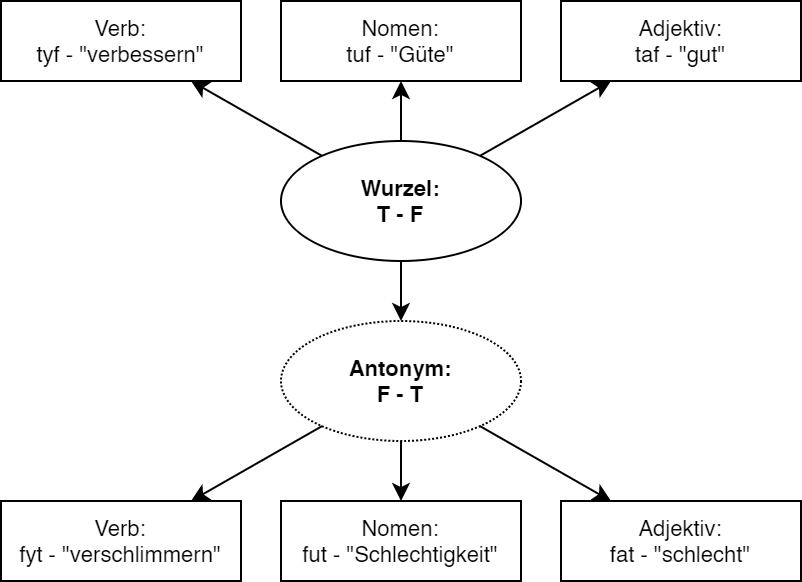
\includegraphics[scale=0.33]{root_derivations_1.png}
	\caption{Ein Diagramm aller Ableitungen der Wurzel ``T-F'' mit Inversion und dem bikonsonantischen Wurzelsystem.}
	\label{root_derivations_1}
\end{figure}

Da das Wurzelsystem nun einen bestimmten Vokal einer bestimmten Wortart zuordnet, können wir ihre ``harten'' Formen verwenden,
um einige semantische Veränderungen anzuzeigen. Ich beschloss, dass die reguläre Form die indikative Stimmung für Verben,
die Singularzahl für Substantive und der positive Grad für Adjektive sein würde. Für die Umlautformen entschied ich mich
für den Imperativ für Verben, den Plural für Substantive und den Superlativ für Adjektive. Dadurch verdoppelt sich die Anzahl
der Formen, die man aus einer einzigen Wurzel extrahieren kann, wie Sie im folgenden Diagramm sehen können.

\begin{figure}
	\centering
	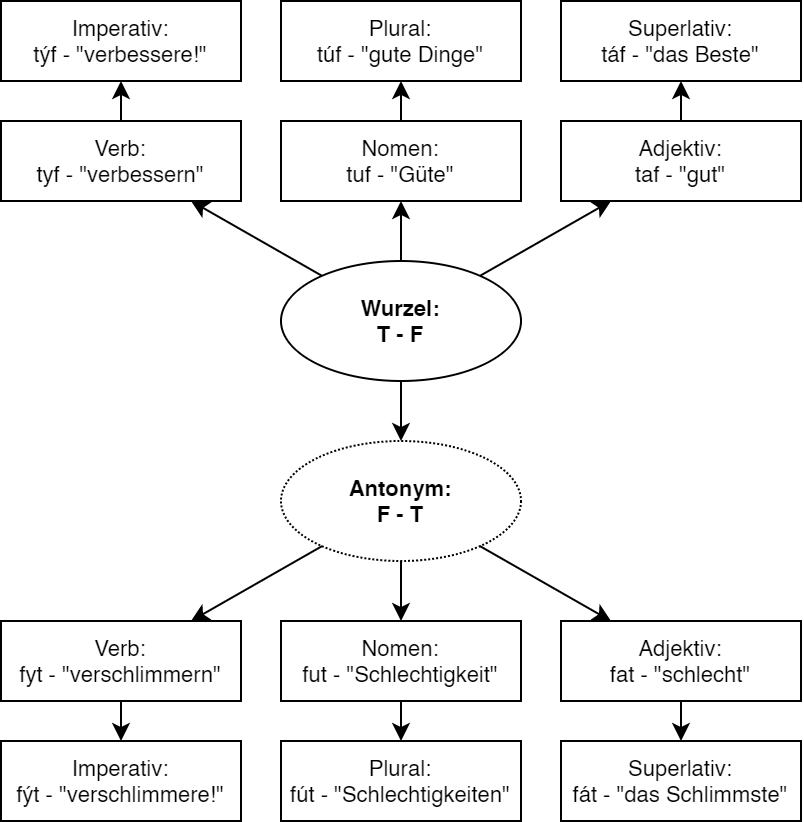
\includegraphics[scale=0.33]{root_derivations_2.png}
	\caption{Ein Diagramm aller Ableitungen der Wurzel ``T-F'' wenn mann die Umlautformen dazufügt.}
	\label{root_derivations_2}
\end{figure}

Danach wollte ich das System noch weiter ausbauen und schuf einige Präfixe, die unabhängig von der Wortart des Wortes
verwendet werden konnten. Diese würden es dem Sprecher ermöglichen, die möglichen Bedeutungen noch zu erweitern.
Zunächst wurden ein Negationspräfix sowie ein Augmentativ und ein Diminutiv hinzugefügt. Da diese auf alle vorhandenen
Ableitungen angewandt und sogar kombiniert werden können, vervielfachte sich die Zahl der möglichen Bedeutungen,
die einem einzigen Wort entnommen werden können, auf 60! Und dabei ist noch nicht einmal berücksichtigt,
dass die meisten Wörter absichtlich mehrdeutig sind, damit sie für mehrere Dinge stehen können. Zunächst war dies recht hilfreich,
um die Anzahl der Wörter zu reduzieren, die ich der Sprache hinzufügen musste, aber es wurde ziemlich schnell klar,
dass dies jeden Lernenden der Sprache nur verwirren würde. Zumal die Haupttaktik bei der Wortbildung darin bestand,
zunächst zu versuchen, das Wort aus anderen Wörtern zusammenzusetzen (z. B. ``Regen'' = ``fallende Flüssigkeit''),
aber obwohl ich in der Tat es geschafft hatte den Wortschatz sehr begrenzt zu halten, glaubte ich nicht, dass irgendjemand ausser mir sie
verstanden hätte. Ich habe dies auch getestet, indem ich meinen Freiwilligen ab und zu zusammengesetzte
Wörter zum Übersetzen vorgelegt habe. Die meisten Antworten bestätigten meine Befürchtungen, so dass ich eine Idee entwickelte,
um die Testkapazität der Sprache zu verbessern und gleichzeitig meine Angst vor dem Hinzufügen neuer Wörter zu überwinden:
Ich würde das Lexikon in kleine Segmente aufteilen, wobei die kleinste Ausgabe der Sprache nur die grundlegenden
grammatikalischen Wörter und eine Handvoll anderer enthalten würde. Danach würde der Umfang des Lexikons allmählich zunehmen,
bis er ein Maximum erreicht, das ich immer noch relativ klein halten wollte. Auf diese Weise könnte ich möglicherweise
Texte in immer kleinere Editionen der Sprache übersetzen, um zu sehen, an welchem Punkt genau sie jeden Anschein von
Bedeutung verliert. Ich beschloss, mir nicht allzu viele Gedanken über die Hinzufügung unnötiger Wörter zu machen,
da ich sie später immer noch einschränken und das Lexikon unterteilen konnte, sobald ich die gesamte Sprache etabliert hatte.
% TODO: Add in here if you do actually finish the Lexicon Size thing

Nachdem diese Grundlage mit dem Gerüst unserer Sprache ausgestattet war, konnte ich mich an die fortgeschritteneren
grammatikalischen Dinge wie Konditionalsätze und Relativsätze machen. Diese habe ich ähnlich wie bei Toki Pona gelöst,
weil es einfach zu verstehen ist und ich keine Zeit damit verschwenden wollte, mir etwas Besseres einfallen zu lassen.
Als ich das Ergebnis hatte, testete ich es an einigen Sätzen und befragte meine Testpersonen, was sie davon hielten und
ob ich ihrer Meinung nach etwas hinzufügen oder entfernen sollte. Sie hatten im Allgemeinen recht wenig Feedback,
und so hielt ich es für den Moment für gut genug und habe lediglich kleine Details verbessert und Wörter hinzugefügt/geändert,
als ich weitere Testsätze schrieb und kurze Texte übersetzte.

\subsection{Prozess der Sprachprüfung}
Zu Beginn des Projekts hatte ich weitaus ehrgeizigere Erwartungen, was das Testen der Sprache anbelangt,
aber im Laufe der Entwicklung wurde klar, dass ich das Testen der Fähigkeiten der Sprache einschränken sollte.
Schon bald wurde das Versuchskonzept auf die folgenden Punkte reduziert: Zuerst würde ich einen grösseren Textblock in die
Sprache übersetzen, danach würde ich meinen Freiwilligen dasselbe Wörterbuch zur Verfügung stellen, das ich für die Übersetzung
verwendet hatte, und ihre Fragen zur Grammatik beantworten, während sie den Text zurück ins Deutsche übersetzten.
Auf diese Weise konnte ich die Sprache testen und verfeinern, indem ich den grösseren Text übersetzte und so herausfand,
wie einfach es ist, die Bedeutung komplexerer Konzepte in der Sprache zu vermitteln, und meine Freiwilligen konnten zeigen,
wie gut man sie verstehen kann. Der Text, für den ich mich schliesslich entschied, war die Geschichte vom ``Turmbau zu Babel''
--- ein Favorit in der conlanging community. Hier ist der vollständige Text der Geschichte auf Deutsch:

\begin{quotation}
    Die ganze Erde hatte eine Sprache und ein und dieselben Worte.
    Als sie ostwärts aufbrachen, fanden sie eine Ebene im Land Schinar und siedelten sich dort an.
    Sie sagten zueinander: Auf, formen wir Lehmziegel und brennen wir sie zu Backsteinen.
    So dienten ihnen gebrannte Ziegel als Steine und Erdpech als Mörtel.
    Dann sagten sie: Auf, bauen wir uns eine Stadt und einen Turm mit einer Spitze bis in den Himmel!
    So wollen wir uns einen Namen machen, damit wir uns nicht über die ganze Erde zerstreuen.
    Da stieg der HERR herab, um sich Stadt und Turm anzusehen, die die Menschenkinder bauten.
    Und der HERR sprach: Siehe, ein Volk sind sie und eine Sprache haben sie alle.
    Und das ist erst der Anfang ihres Tuns. Jetzt wird ihnen nichts mehr unerreichbar sein, wenn sie es sich zu tun vornehmen.
    Auf, steigen wir hinab und verwirren wir dort ihre Sprache, sodass keiner mehr die Sprache des anderen versteht.
    Der HERR zerstreute sie von dort aus über die ganze Erde und sie hörten auf, an der Stadt zu bauen.
    Darum gab man der Stadt den Namen Babel, Wirrsal, denn dort hat der HERR die Sprache der ganzen Erde
    verwirrt und von dort aus hat er die Menschen über die ganze Erde zerstreut.\citep{Bibel2020}
\end{quotation}

Ursprünglich hatte ich auch geplant, Testgespräche mit meinen Freiwilligen zu führen,
aber sie waren zu dieser Zeit viel zu sehr mit ihren eigenen Projekten beschäftigt, um eine ganze Sprache zu lernen,
und wir konnten uns während der Pandemie nicht mehr treffen. Hätten wir es dennoch getan, wäre meine ursprüngliche
Idee für das Experiment gewesen, eine kurze Zeit unseres normalen Lebens damit zu verbringen,
die grundlegenden Dinge zu beschreiben, die wir tun, und uns normal in der Sprache zu unterhalten.
Das wäre meiner Meinung nach der beste Weg gewesen, um die Fähigkeit der Sprache zu testen, alltägliche Dinge auszudrücken.
Das System des skalierenden Lexikons könnte auch verwendet werden, indem man die Konversation zunächst auf das kleinste
Lexikon beschränkt und den Umfang allmählich erhöht, bis der Punkt erreicht ist, an dem es Sinn macht, oder umgekehrt.

\subsection{Prozess der Erstellung der Orthografie}
Ursprünglich hatte ich geplant, die Erstellung der Orthographie bis zum Ende des Projekts aufzuschieben,
als zusätzlichen Bonus für den Fall, dass noch Zeit übrig bliebe, aber ich schaffte es,
so viel von der Sprache so schnell zu erstellen, dass meine Liebe zu Schriftsystemen die Oberhand gewann und ich begann,
an einigen Konzepten zu arbeiten. Die ersten Ideen, die ich hatte, waren von Systemen wie Devanagari und Arabisch inspiriert,
die die Vorteile der sehr systematisch organisierten Phonologie und Phonotaktik der Sprachen hätten nutzen können,
um kompaktere Glyphen zu schaffen, aber davon wurde mir von meinen Freiwilligen abgeraten, die keine Lust hatten,
das Schriftsystem mühsam zu lernen. Schließlich entschied ich mich für ein Alphabet, bei dem diakritische Zeichen
die Aussprache beeinflussen. Dies führte zu einem System, bei dem ich nur 8 eindeutige Symbole mit einer Handvoll
diakritischer Zeichen benötigte, um alle 18 in der Sprache vorhandenen Laute darzustellen. Nachdem ich die grundlegenden
Glyphenentwürfe hatte, wurden sie unzählige Male überarbeitet, bis sie einen Punkt erreichten, an dem ich sie für praktisch,
eindeutig und ästhetisch ansprechend hielt.

Während der Iterationsphase erstellte ich eine einfache Schriftart für die Sprache,
die zugegebenermaßen nicht besonders schön war, aber sie ermöglichte es, die Sprache digital darzustellen.
Ich habe meinen Entwurf für eine fast vollständige Version des Schriftsystems sogar in einem Internetforum
für die Erstellung von Orthographien gepostet, was mir einige gute Rückmeldungen zu den Designentscheidungen
und sogar eine weitere Schriftart einbrachte, die jemand kostenlos dafür anfertigte! Leider habe ich sie aus
urheberrechtlichen Gründen und aufgrund der Tatsache, dass sich die Schrift danach weiterentwickelt hat,
nicht weiter verwendet, aber sie war dennoch recht bemerkenswert. Die Schriftart die für die Textausschnitte
in Anhang C verwendet wurde habe ich selber gemacht. Ich wollte ursprünglich einen Text von Hand, ganz
kalligraphisch ausschreiben um die Kunst der Sprachentwicklung ein wenig zu zeigen, aber dafür fehlte auch die Zeit.

Jetzt, wo sich die Vertiefungsarbeit dem Ende zuneigt, könnte ich mir überlegen, ob ich nicht noch ein paar
kompliziertere Schriftsysteme dafür entwickeln sollte, einfach nur so zum Spaß. Es könnte eine viel dekorativere
Form des Schreibens sein, die mehr Gebrauch von der starren Phonologie macht, oder ich könnte sogar ganz praktisch
eine Logographie machen, was während des Projekts aufgrund der Zeitbeschränkungen unmöglich war.
Es wäre aber immer noch ein recht effizientes System, wenn man bedenkt, wie wenige Wörter es zu lernen gibt,
und wie viele lange zusammengesetzte Wörter in der Sprache oft auftauchen.




\section{Resultate und Schlussfolgerungen}
\subsection{Resultate des Experiments}
%TODO%


\subsection{Kapazität der Sprache}
%TODO%


\subsection{Schlussfolgerungen zur Spracherstellung}
%TODO%




\section{Lernjournal \& Reflexion}
\subsection{Lernjournal}
%TODO%

\subsection{Reflexion über die VA}
%TODO%




\bibliography{Bibliography}
\bibliographystyle{apalike}

\renewcommand{\section}[1]{\newpage\vspace*{\fill}\Huge{#1}\vspace*{\fill}}

%\section{Anhang A: Projektbeschrieb}
%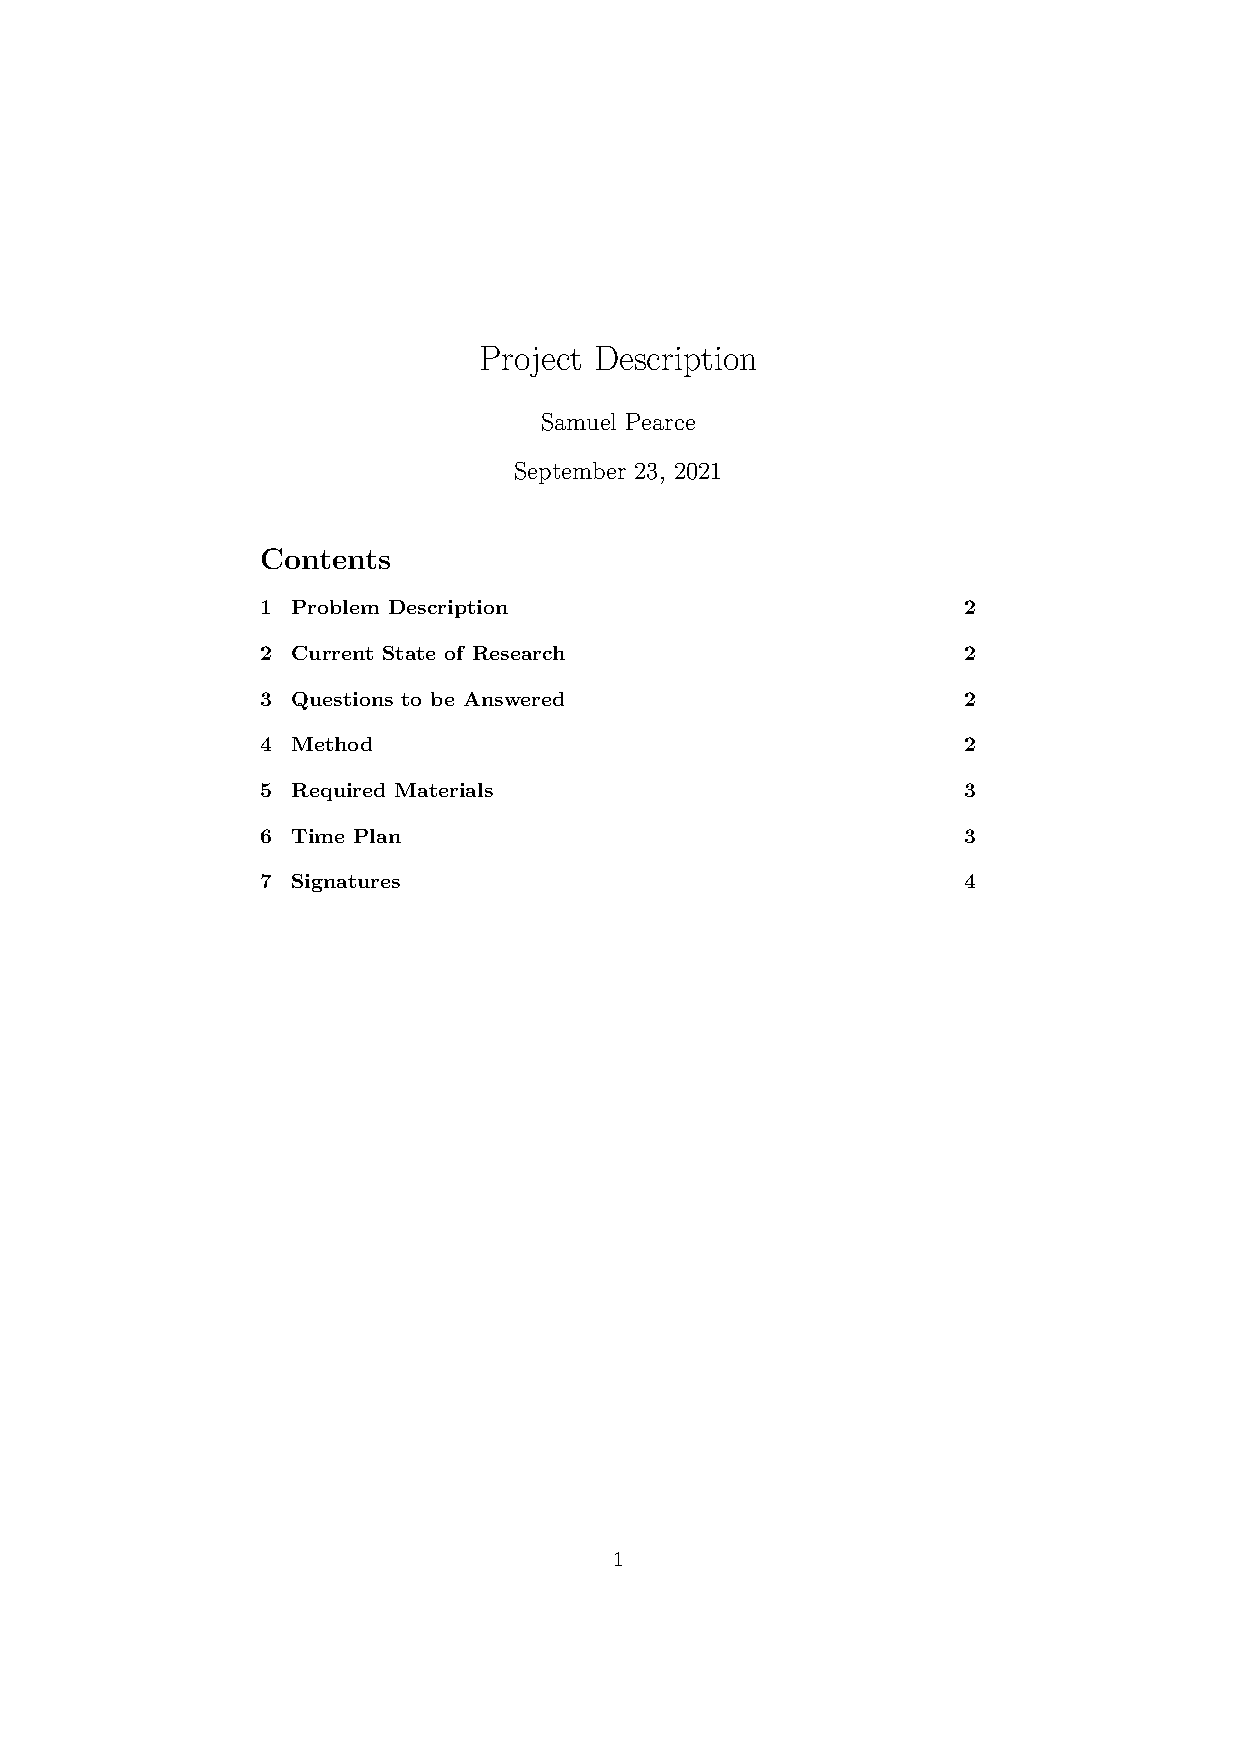
\includepdf[pages=-]{../Project_Description/Project_Description.pdf}

%\section{Anhang B: Sutlun Grammatik und Lexikon}
%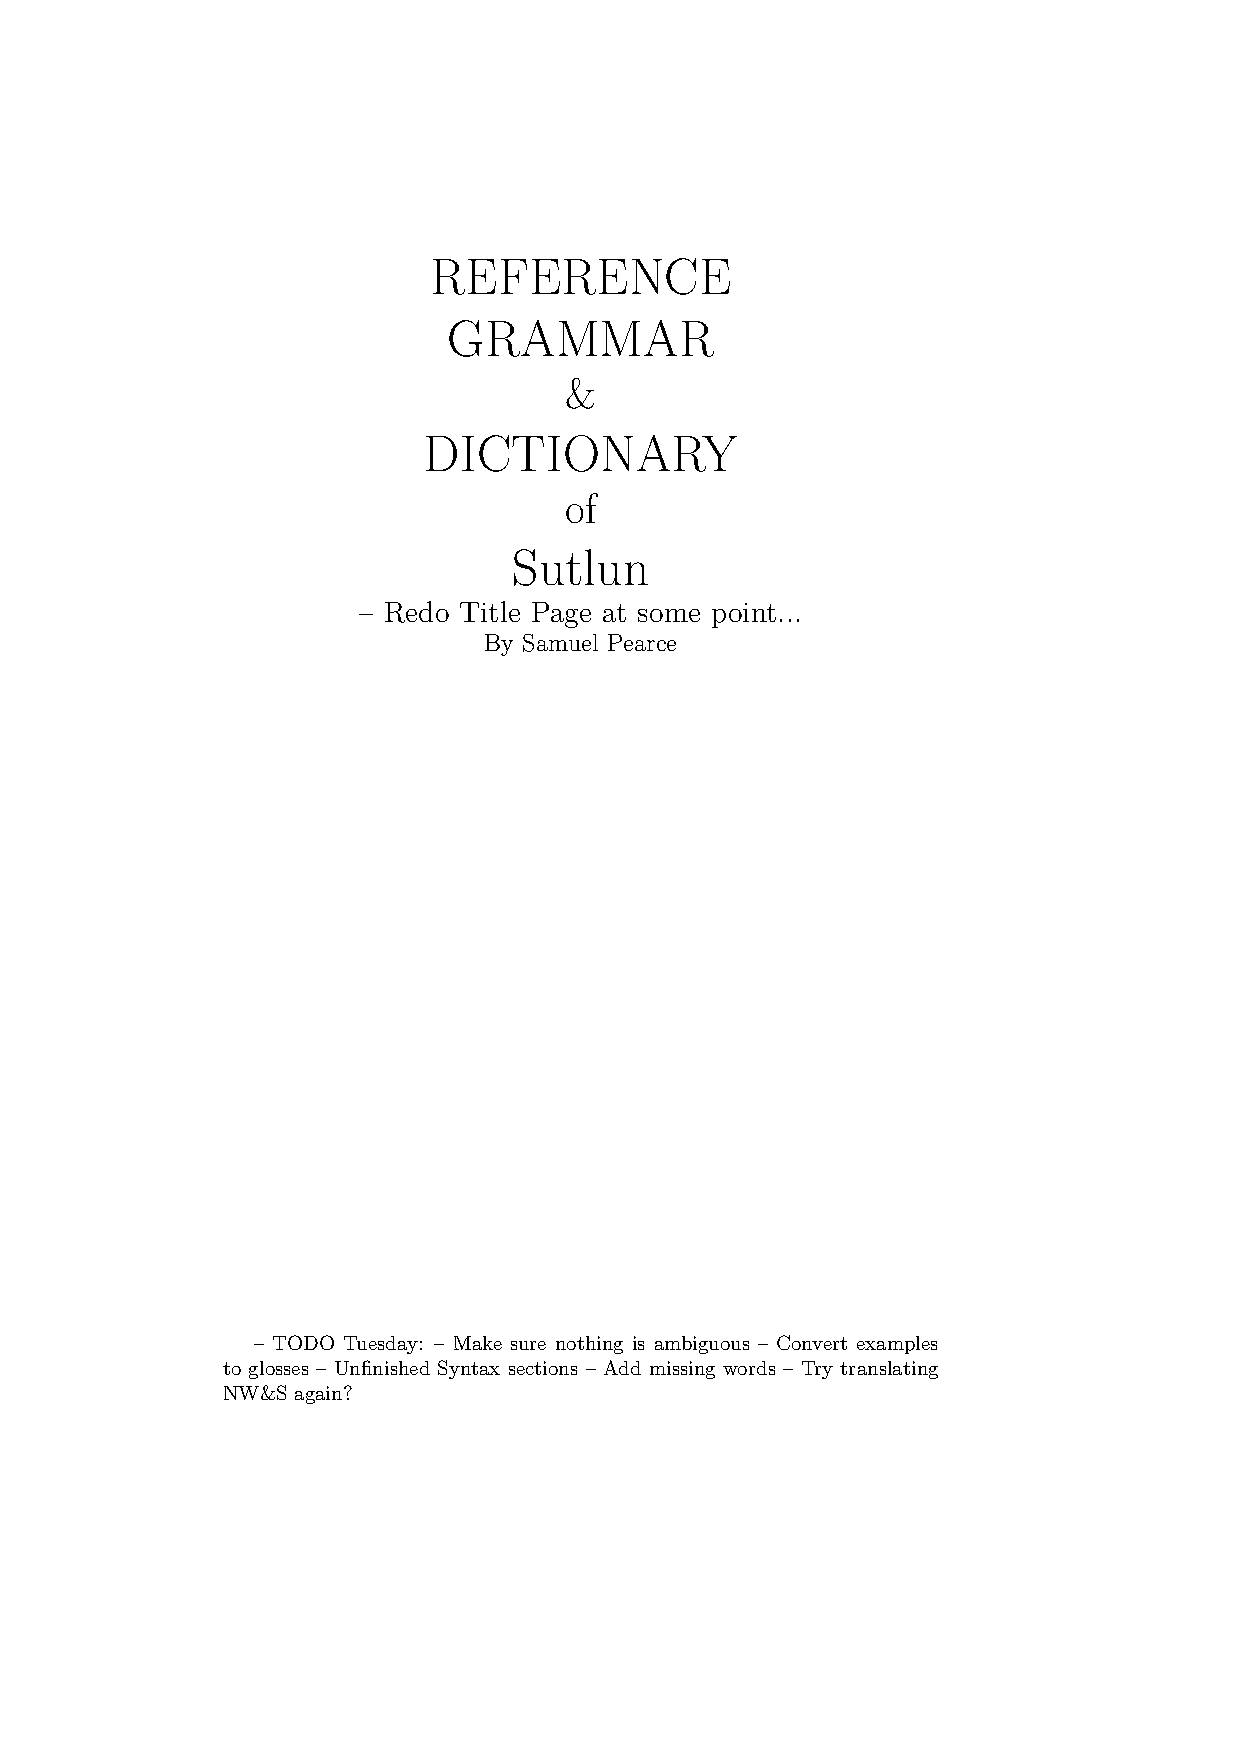
\includepdf[pages=-]{../Sutlun_Grammar/Sutlun_Grammar.pdf}

%\section{Anhang C: Übersetzte Texte}
%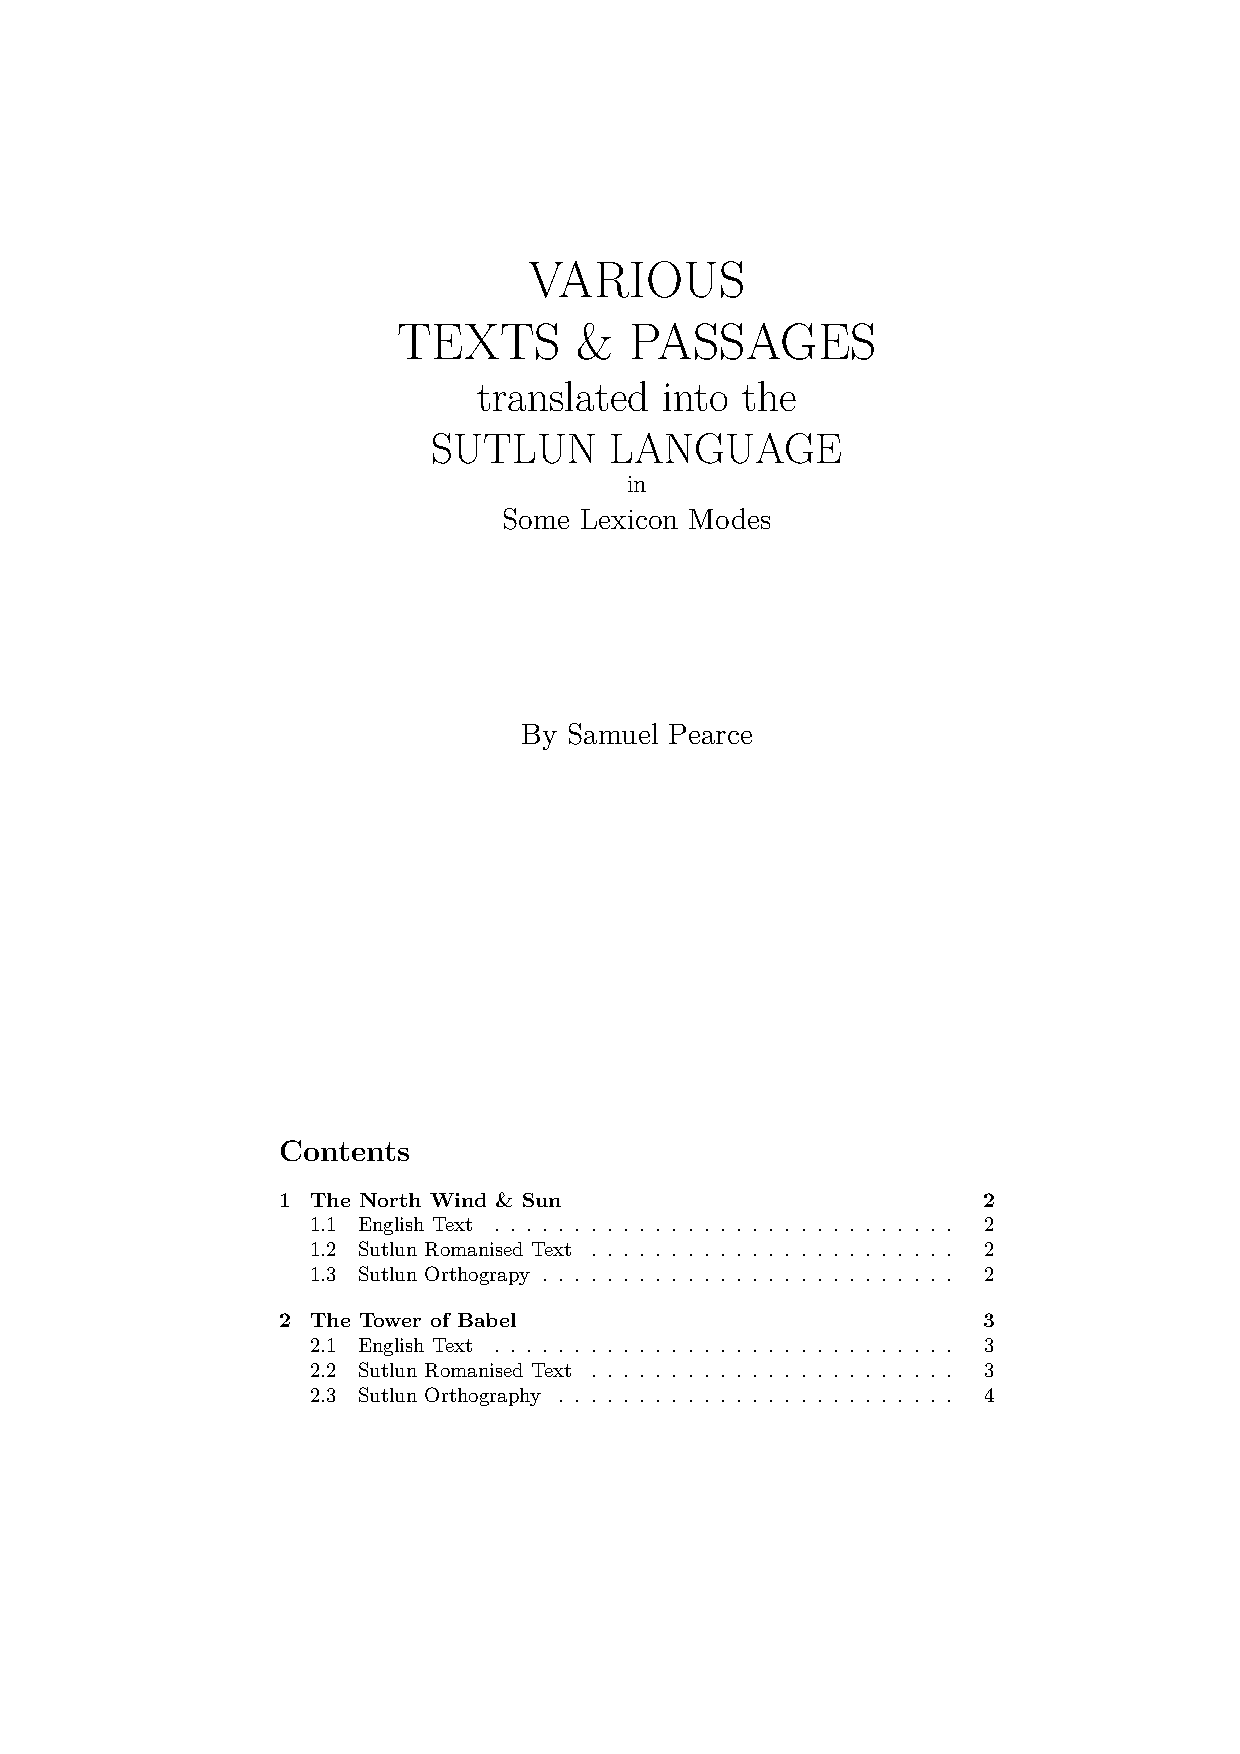
\includepdf[pages=-]{../Text_Translations/Text_Translations.pdf}

%\section{Anhang D: Arbeitsprotokoll}
%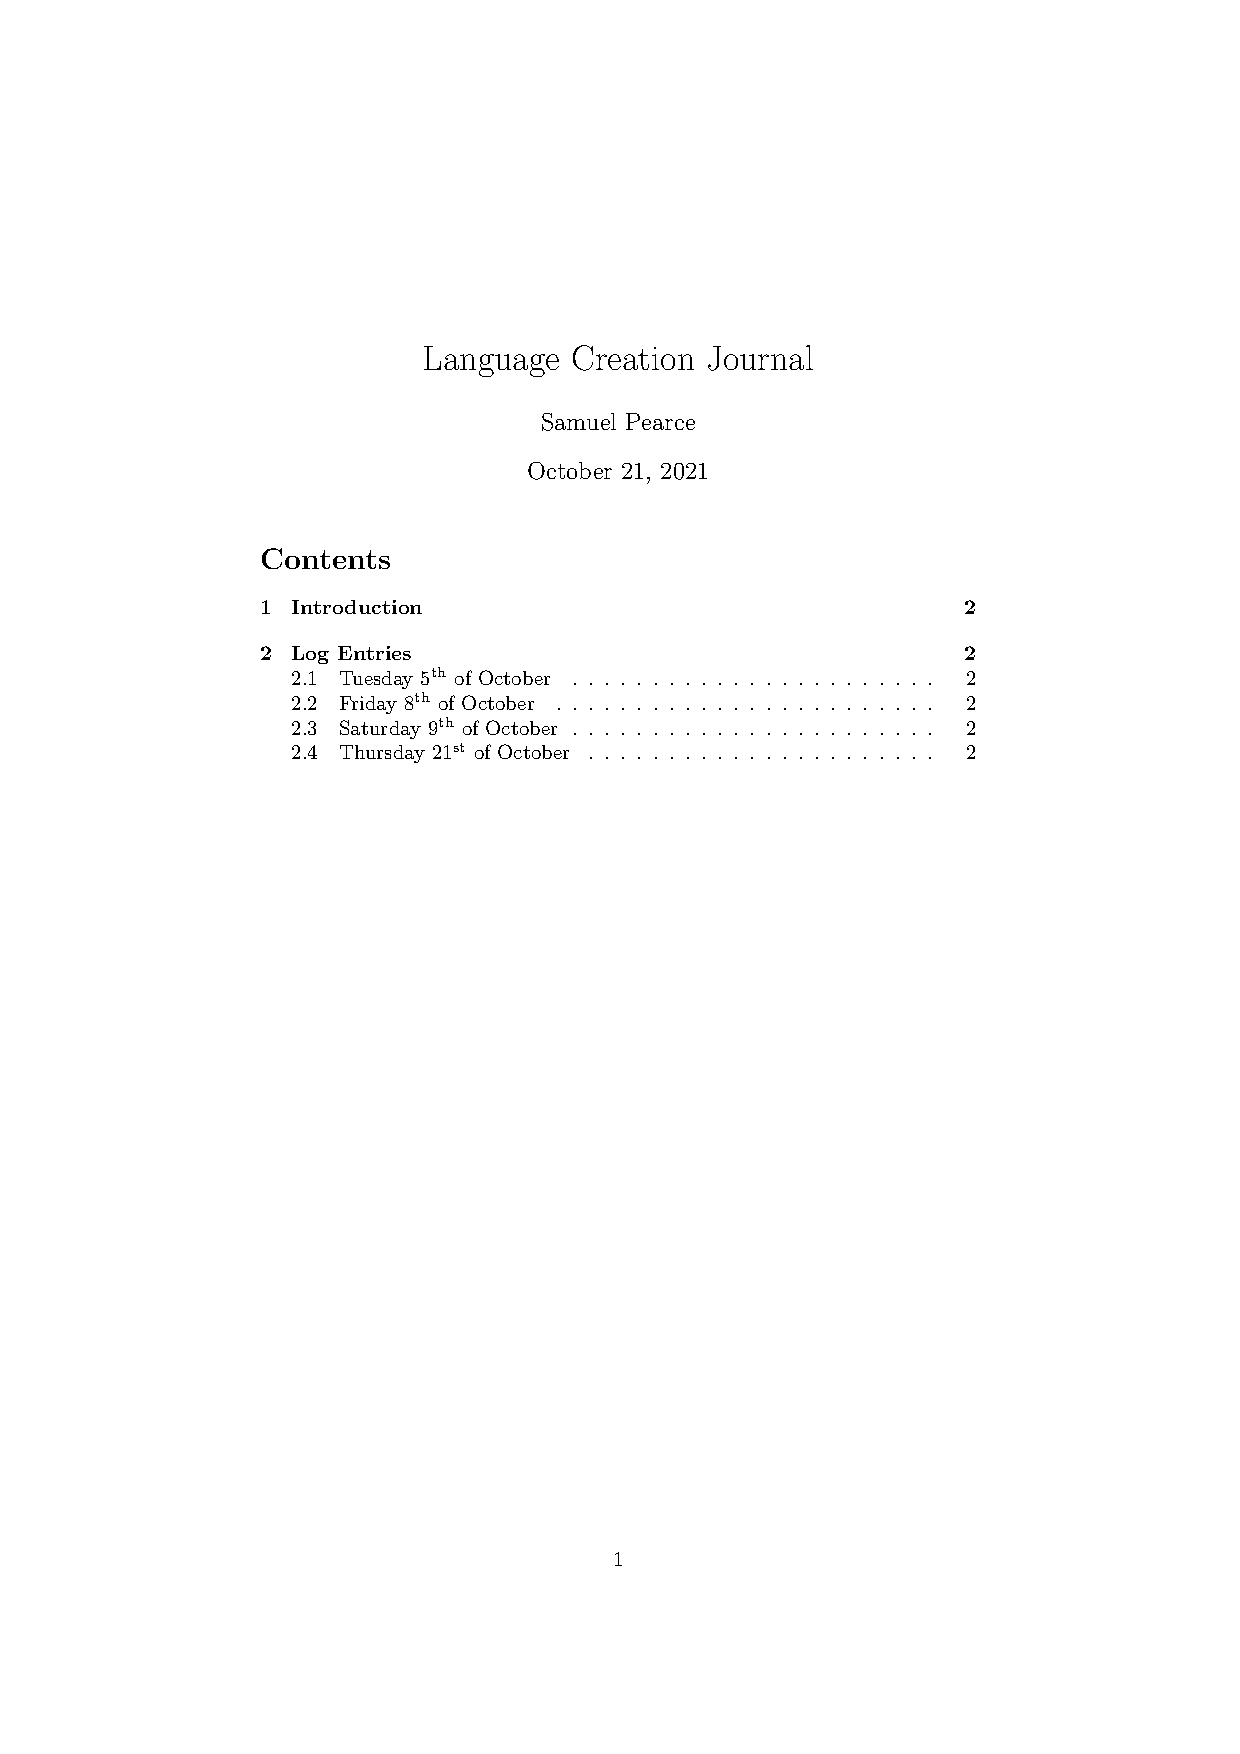
\includepdf[pages=-]{../Language_Log/langlog.pdf}

%\section{Anhang E: Urheberrechtserklärung}
%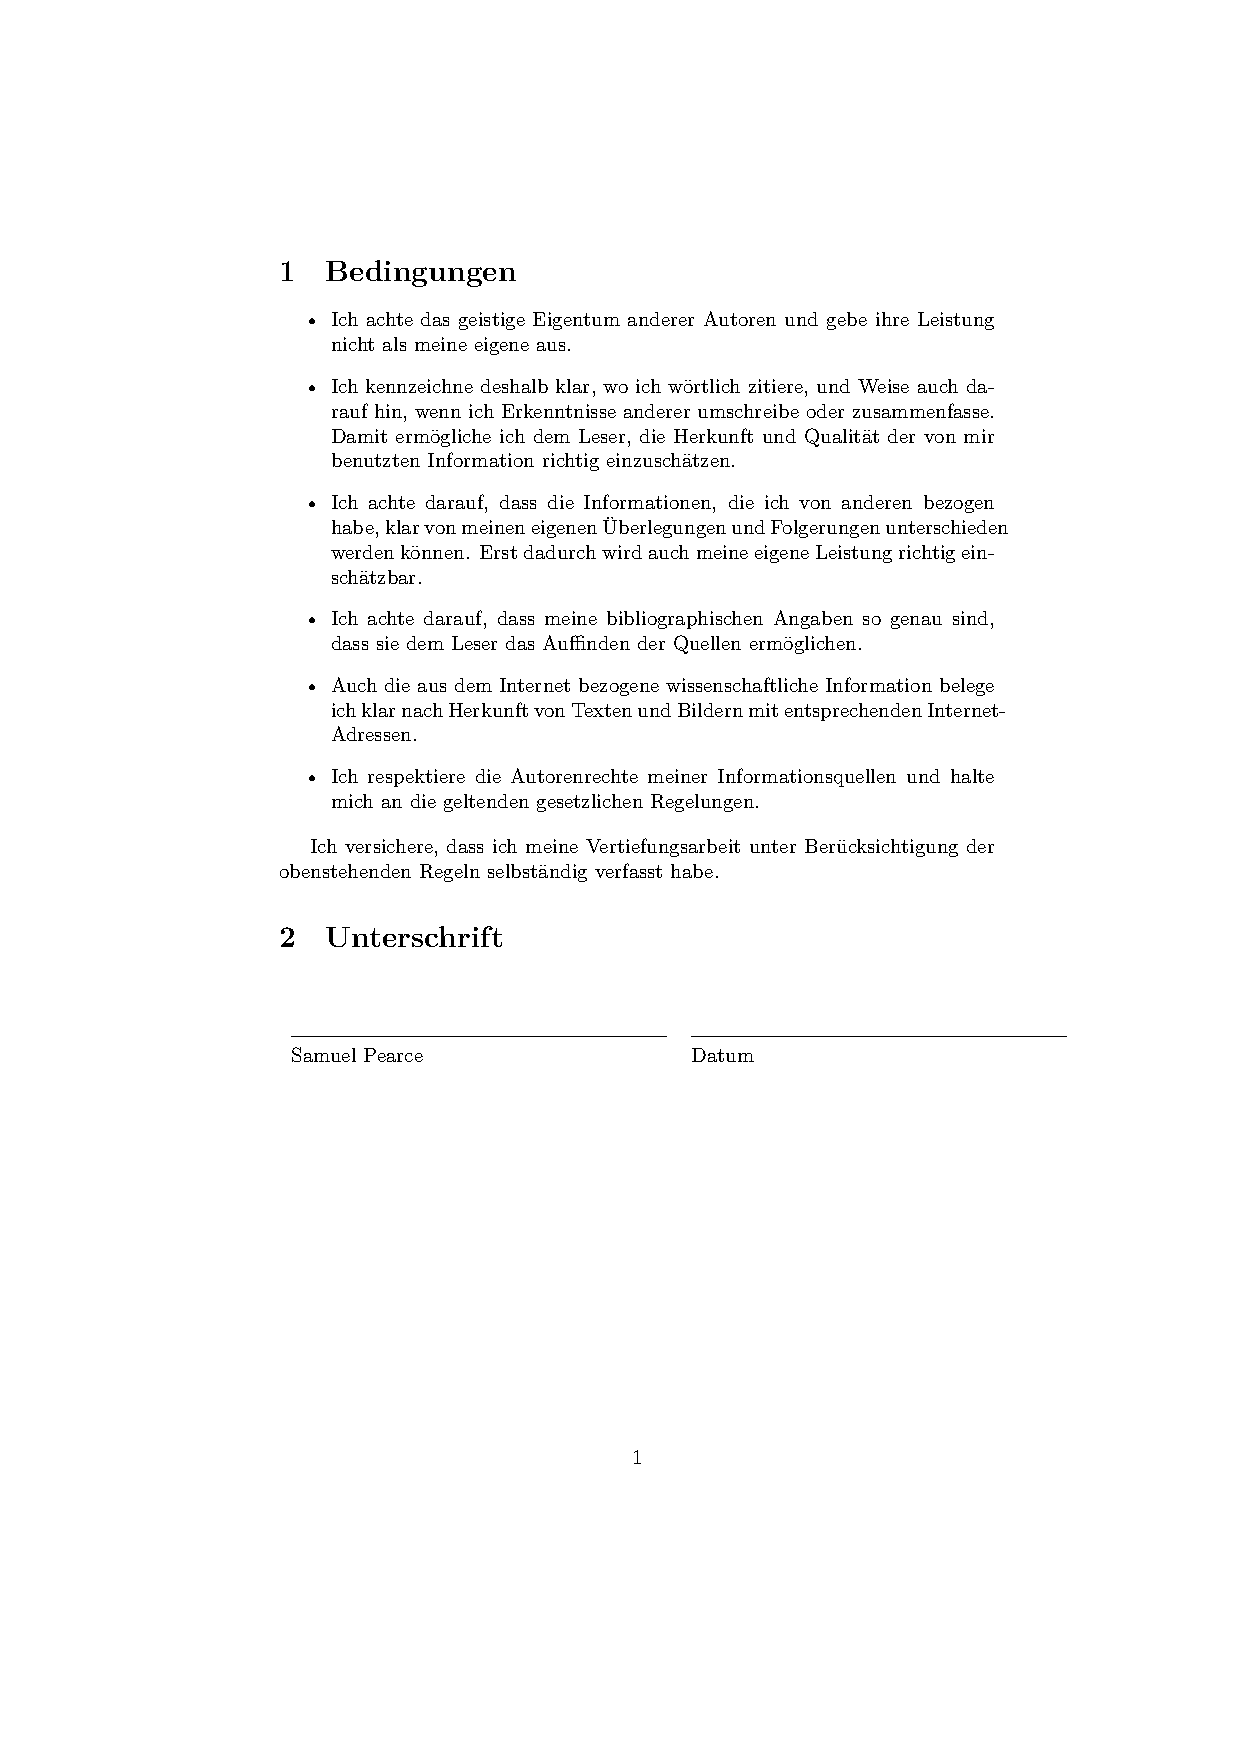
\includepdf[pages=-]{../Copyright_Declaration/Copyright_Declaration.pdf}

\end{document}